\documentclass{article}
\usepackage{titlesec}
\usepackage[utf8]{inputenc}
\usepackage[a4paper, total={6in, 9in}]{geometry}
\usepackage{fancyhdr}
\usepackage{graphicx} % Add the graphicx package
\usepackage{lipsum} % For placeholder text
\usepackage{tikz}
\usepackage{cite}
\usepackage{bm}
\usepackage{acronym}
\usepackage{amsmath,amssymb,amsfonts}
\usepackage{algorithmic}
\usepackage{graphicx}
\usepackage{caption}
\usepackage{subcaption}
\captionsetup{font=small, labelfont=bf}
\captionsetup[sub]{labelsep=period, subrefformat=brace}
\usepackage{tikz}
\usepackage{textcomp}
\usepackage{xcolor}
\usepackage[numbers]{natbib}
\bibliographystyle{ieeetrann}
\usepackage{subfig}
\usepackage{svg}
\usepackage{tikz,pgfplots,pgfplotstable}
\pgfplotsset{compat=1.9} % set to 1.8 to get old behaviour
\usepackage{subfigure}
\usepackage{paralist}
\usepackage{longtable}

% Set up page headers and footers
\pagestyle{fancy}
\fancyhf{}
\rhead{ }
\rhead{team MOSFETS}
\lhead{Metroband - The Metronome Wristband}
\cfoot{\thepage}

% Redefine the abstract environment to be single column
\renewenvironment{abstract}
{\par\noindent\textbf{\abstractname}\ \ignorespaces}{\par}

% Redefine section format
\titleformat{\section}
{\normalfont\Large\bfseries}{\thesection}{1em}{}

\begin{document}
	
	% Cover Page
	\begin{titlepage}
		
		\centering
		\vspace*{0.5cm}
		
\includegraphics[width=5cm]{logo.png} % Replace with the path to your university logo
		\par\vspace{0.02cm}
		Department of Electronic \& Telecommunication Engineering
  
            University of Moratuwa, Sri Lanka.
		\par\vspace{4cm}
		{\LARGE\bfseries Project Report:}\\{\LARGE Metroband - The Metronome Wristband\par}
		\vspace{4cm}
		\begin{tabular}{l l}
			& \\
            \multicolumn{2}{c}{\textbf{team MOSFETS}}\\
            210415N	&	Navarathne D.M.G.B.\\
            210594J &	Senevirathne I.U.B.\\
            210608J &	Silva L.J.J.P.\\
            210609M	&	Silva M.K.Y.U.N. \\
		\end{tabular}\\
		\vspace{1.3cm}
            {Submitted in partial fulfillment of the requirements for the module\par}
		{EN 1190 Engineering Design Project\par}
	
		\vspace{0.5cm}
		{\large 06/08/2024\par}
		\vfill
	\end{titlepage}

        \newpage
        \tableofcontents
	\newpage
	
        \section{Introduction}
        The aim of this project is to design and develop a pulsating wristband according to a given BPM to give a better experience for beginner, intermediate or professional musicians. This project is undertaken by a team of four engineering undergraduates from the University of Moratuwa. The following report provides details of the progress made towards achieving the project objectives.
        
        \subsection{The Problem, and the Motivation to Solve it}
        \subsubsection{Problem Definition}
        In music, BPM is the speed of a musical piece. It determines the overall energy and the feel of the musical performance. It is measured in Beats per Minute (BPM). In practicing to master a piece, it is crucial for one to be able to play it in time. This is even more important when playing in groups, where the whole group must play it at the same BPM. It is often maintained throughout the music using a metronome, in-ear headphones, or a conductor.\\

        One of the major problems of musicians of both beginner and amateur levels, and sometimes even professionals is, keeping up the BPM while performing or practicing. For beginners, it brings great frustration as well as for many others when performing with a group it ruins the entire timing of the song. This often wastes a good fraction of the practice time.\\

        There are a few solutions to combat this. Namely:
        \begin{compactitem}
                \item Metronomes
                \item In-ear Headphones
        \end{compactitem}
        .\\
        But they too have their own potential problems and limitations which are listed below that have been complained about by many users:

        \begin{itemize}
                \item \textbf{External noise:} In noisy environments, metronomes can be hard to hear, and in-ear headphones can isolate the player from outside sounds, making it challenging to play with others.
                \item \textbf{Distraction:} Some musicians may find metronomes to be distracting or irritating, especially if they are practicing for extended periods of time. Over time, in-ear headphones may also result in ear discomfort or tiredness.
                \item \textbf{Inaccessibility:} Due to physical constraints or disabilities like hearing impairments, some musicians may find it challenging to utilize conventional metronomes or headphones, which have been recognized as a major issue.
                \item \textbf{Cost:} Metronomes and in-ear headphones can be expensive which will not make it feasible for many users.
        \end{itemize}

        \subsubsection{Motivation for our solution}
        Since all our group members are practicing music up to some extent, we have all felt the need of addressing this problem. However, to gather more information about this matter we carried out an online survey which spanned out not only through local music societies but also across multiple global music societies as well. The communities from which we gathered information are as follows:

        \begin{compactitem}
                \item Classical Music Society (CMS) of the University of Moratuwa
                \item Discord servers such as ‘We are engineers’ of Mattias Krantz and ‘RoomieOfficial’ of Joel Berghult; two popular Swedish music YouTubers
                \item Peer musician groups
                \item Social media such as X (formerly Twitter) and Facebook
                \item Personal contacts
        \end{compactitem}

        \newpage
        The results of our survey are as follows:

        \begin{figure}[htpb]
            \centering
            \begin{minipage}{0.45\textwidth}
                \centering
                \begin{subfigure}{\textwidth}
                    \centering
                    \begin{tikzpicture}
                        \begin{axis}[
                            ybar stacked,
                            width=7cm,
                            xlabel={Categories},
                            ylabel={Values},
                            legend style={at={(0.5,-0.65)}, anchor=north, legend columns=2},
                            symbolic x coords={Very Hard, Hard, Neutral, Easy, Very Easy},
                            xtick=data,
                            x tick label style={rotate=45, anchor=east, xshift=-1.5mm, yshift=-2mm},
                            nodes near coords={},
                            nodes near coords align={vertical},
                            ]
                            \addplot+[bar width=0.4cm] coordinates {(Very Hard, 0) (Hard, 1) (Neutral, 3) (Easy, 0) (Very Easy, 2)};
                            \addplot+[bar width=0.4cm] coordinates {(Very Hard, 2) (Hard, 3) (Neutral, 7) (Easy, 6) (Very Easy, 0)};
                            \addplot+[bar width=0.4cm] coordinates {(Very Hard, 1) (Hard, 4) (Neutral, 18) (Easy, 27) (Very Easy, 7)};
                            \addplot+[bar width=0.4cm] coordinates {(Very Hard, 0) (Hard, 0) (Neutral, 1) (Easy, 4) (Very Easy, 1)};
                            \legend{Played in past, Beginner, Intermediate, Professional}
                        \end{axis}
                    \end{tikzpicture}
                \end{subfigure}
            \end{minipage}
            \hspace{1cm}
            \begin{minipage}{0.45\textwidth}
                \centering
                \begin{subfigure}{\textwidth}
                    \centering
                    \begin{tikzpicture}
                        \begin{axis}[
                            ybar stacked,
                            width=7cm,
                            xlabel={Categories},
                            ylabel={Values},
                            legend style={at={(0.5,-0.65)}, anchor=north, legend columns=2},
                            symbolic x coords={Very Ineffective, Ineffective, Neutral, Effective, Very Effective},
                            xtick=data,
                            x tick label style={rotate=45, anchor=east, xshift=-1.5mm, yshift=-2mm},
                            nodes near coords={},
                            nodes near coords align={vertical},
                            ]
                            \addplot+[bar width=0.4cm] coordinates {(Very Ineffective, 1) (Ineffective, 1) (Neutral, 2) (Effective, 0) (Very Effective, 0)};
                            \addplot+[bar width=0.4cm] coordinates {(Very Ineffective, 1) (Ineffective, 0) (Neutral, 4) (Effective, 4) (Very Effective, 2)};
                            \addplot+[bar width=0.4cm] coordinates {(Very Ineffective, 6) (Ineffective, 8) (Neutral, 3) (Effective, 17) (Very Effective, 14)};
                            \addplot+[bar width=0.4cm] coordinates {(Very Ineffective, 0) (Ineffective, 0) (Neutral, 1) (Effective, 1) (Very Effective, 4)};
                            \legend{Played in past, Beginner, Intermediate, Professional}
                        \end{axis}
                    \end{tikzpicture}
                \end{subfigure}
            \end{minipage}
            \caption{Comparison of Stacked Bar Charts A and B}
        \end{figure}

        \subsection{Our Solution}
        As a solution to these critical problems and limitations that have arisen, after thorough observation and research, we have decided that the best solution would be a wristband that is pulsating according to a given BPM which we named \textbf{‘Metroband’}. The reasonings for our solution are listed as follows:

        \begin{itemize}
                \item \textbf{Convenience:} A wristband is portable and wearable, so it can be used anywhere and anytime without the need for a separate device. This can be especially useful for musicians who need to maintain a consistent BPM while on the go, such as during rehearsals or performances.
                \item \textbf{Discreetness:} A vibrating wristband produces a subtle, tactile cue that only the wearer can feel, unlike a metronome which produces an audible sound that can be distracting or disruptive in certain settings, such as recording studios or quiet performance venues.
                \item \textbf{Personalization:} A wristband can be personalized to the user's preferences, allowing them to set their own BPM and adjust the intensity of the vibrations to match their playing style or musical genre.
                \item \textbf{Accessibility:} A wristband can be a useful tool for musicians with hearing impairments or who prefer to play without auditory distractions, as it provides a non-auditory way to keep track of the BPM.
        \end{itemize}

        \section{Technical feasibility}
        The physical appearance of the Metroband would be similar to a smartwatch which could be easily worn on the wrist with simply one knob to do all the operations. Moving onto the internal structure of the Metroband, it is basically built around a single dual-core microcontroller that takes inputs from the knob and displays the relevant BPM on an LCD display. All these devices are powered by a rechargeable Lithium-Ion battery.\\
        
        The required components such as ESP32, rotary encoders, LCD TFT displays, MCP73831 are readily available on the market, both on online vendors as well through local sellers. Further, thorough documentation of these components is available online.\\
        
        We have planned on to programme the ESP32 using another ESP32 Development Kit, using the Arduino IDE. Due to the availability of well optimized free and open-source libraries, the implementation of Bluetooth can be done way far more efficiently.

        \section{Product Architecture}
        Below shown is a block diagram of the abstract modules in the Metroband. It has clearly mentioned the connections, data flow directions, and some data on what data are communicated between the modules that  are described earlier.

            \begin{figure}[!htb]
                \centering
                \begin{tikzpicture}
                    \node at (0.5,-0.2){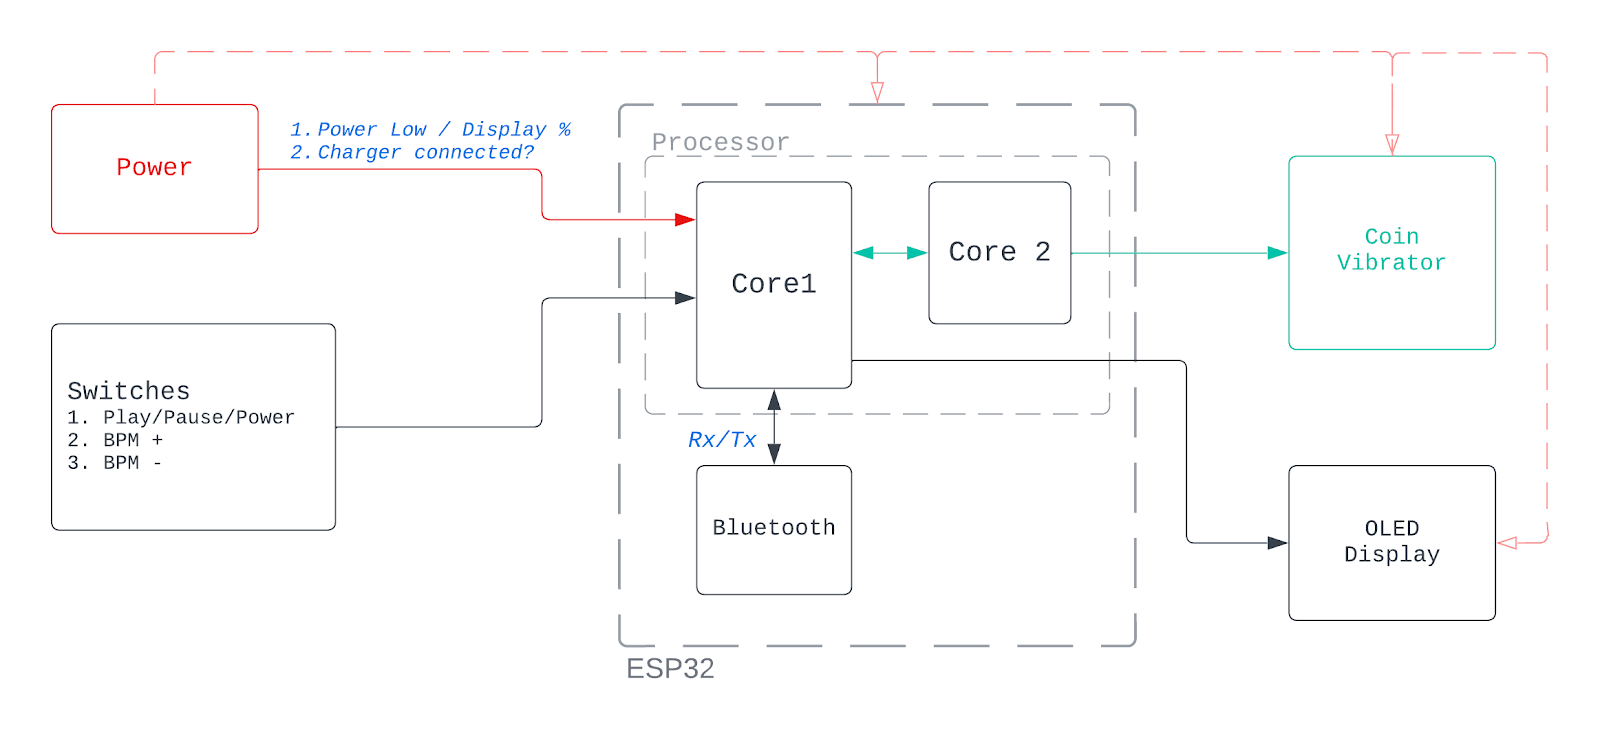
\includegraphics[width=15.5cm]{1.png}};
                \end{tikzpicture}
                \caption{Product architecture}
            \end{figure}

        Functionalities of each module is as follows:
        \subsection{ESP32 Micro-controller}
        This is the microcontroller that we will be using for our product. Each operation is split into tasks, and the ESP32 executes them according to the priority set by the code. Also, the Bluetooth module allows the device to communicate with the mobile app.

        \subsection{Switches}
        As the switch we are using a rotary encoder. Mainly because it can be used to many functionalities. By rotating it clockwise and counterclockwise, we can increase or decrease the BPM. By pressing and depressing it, we can play/pause sending pulses to the vibrating motor. Long press will switch on/off the devices.

        \subsection{LCD TFT Display}
        This will be the display used to mainly show the BPM. Other than that, it will show the Bluetooth connectivity and battery percentage as well.

        \subsection{Coin Vibrator}
        This is the vibrating motor used in our device. It vibrates according to the pulses sent by the microcontroller. In fact, the pulses will be sent through a transistor in switch mode which will give the full power of the battery to the motor.

        \subsection{Power}
        We will be using a rechargeable Lithium-Ion battery to power up all the devices in our product. To handle the charging process, there will be charging IC as well.

        \section{Sketches}
        \subsection{Initial Sketches}
            \begin{figure}[!htb]
                \centering
                \begin{tikzpicture}
                    \node at (0.5,-0.2){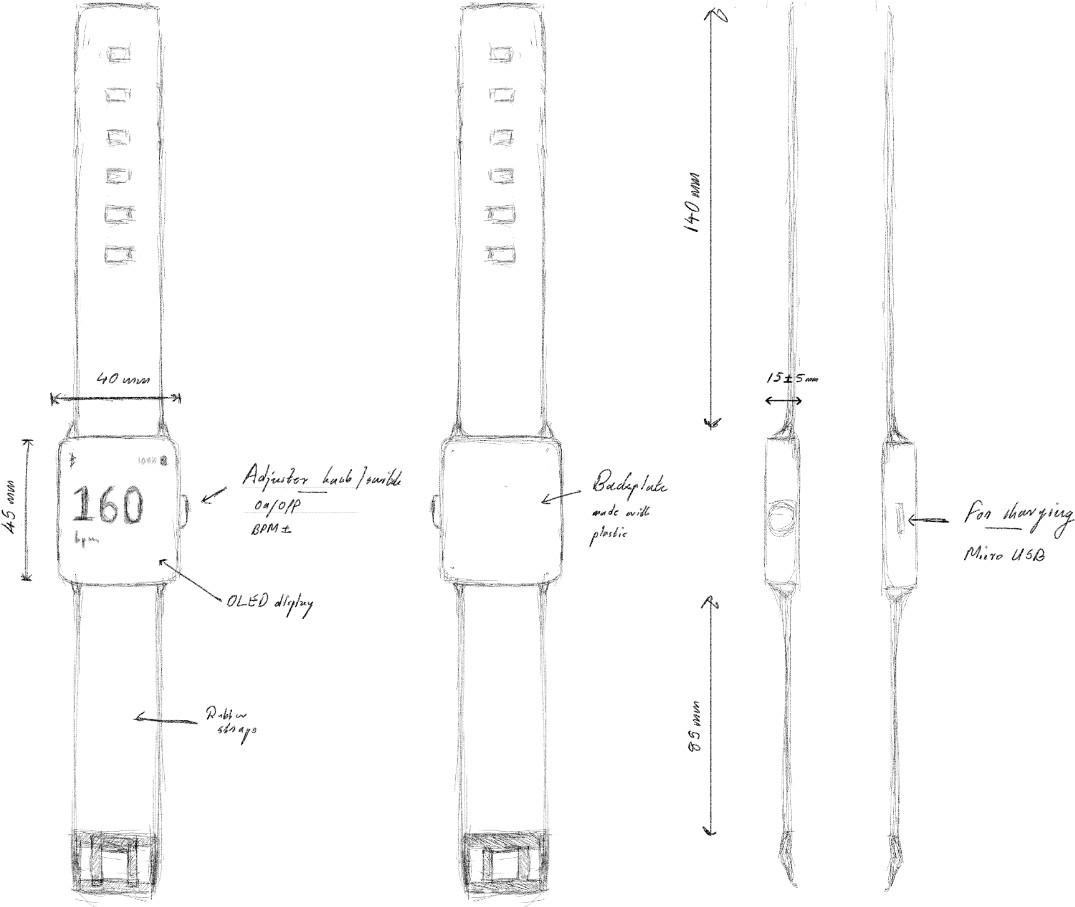
\includegraphics[width=15cm]{2.jpeg}};
                \end{tikzpicture}
                \caption{Initial sketch}
            \end{figure}

        \subsection{Final Design}

        \begin{minipage}{\linewidth}
                \centering
                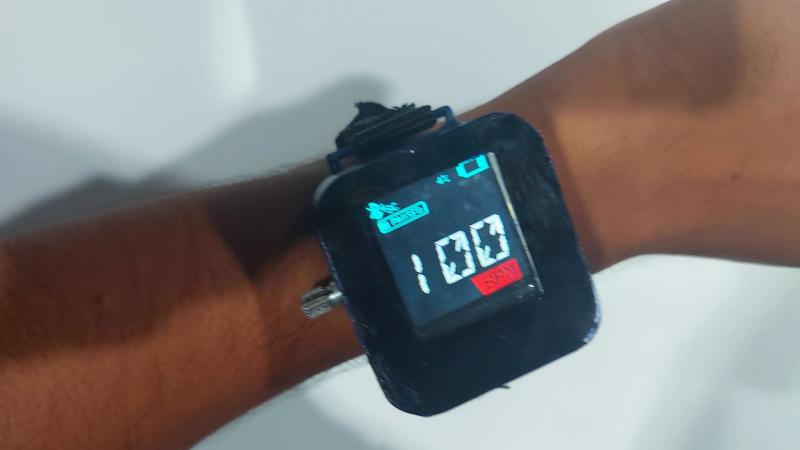
\includegraphics[height=0.25\linewidth]{6.jpeg}
                \hspace{0.005\linewidth}
                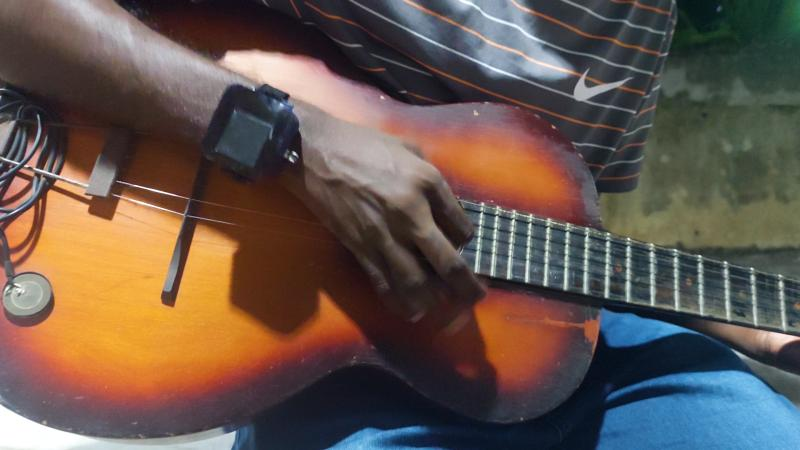
\includegraphics[height=0.25\linewidth]{7.jpeg}
                \captionsetup{justification=centering} % Center-align the caption
                \captionof{figure}{Final design, worn on hand}
            \end{minipage}

        \section{Finalized Project Details}
        \subsection{Schematic and PCB}
        \begin{figure}[!htb]
                \centering
                \begin{tikzpicture}
                    \node at (0.5,-0.2){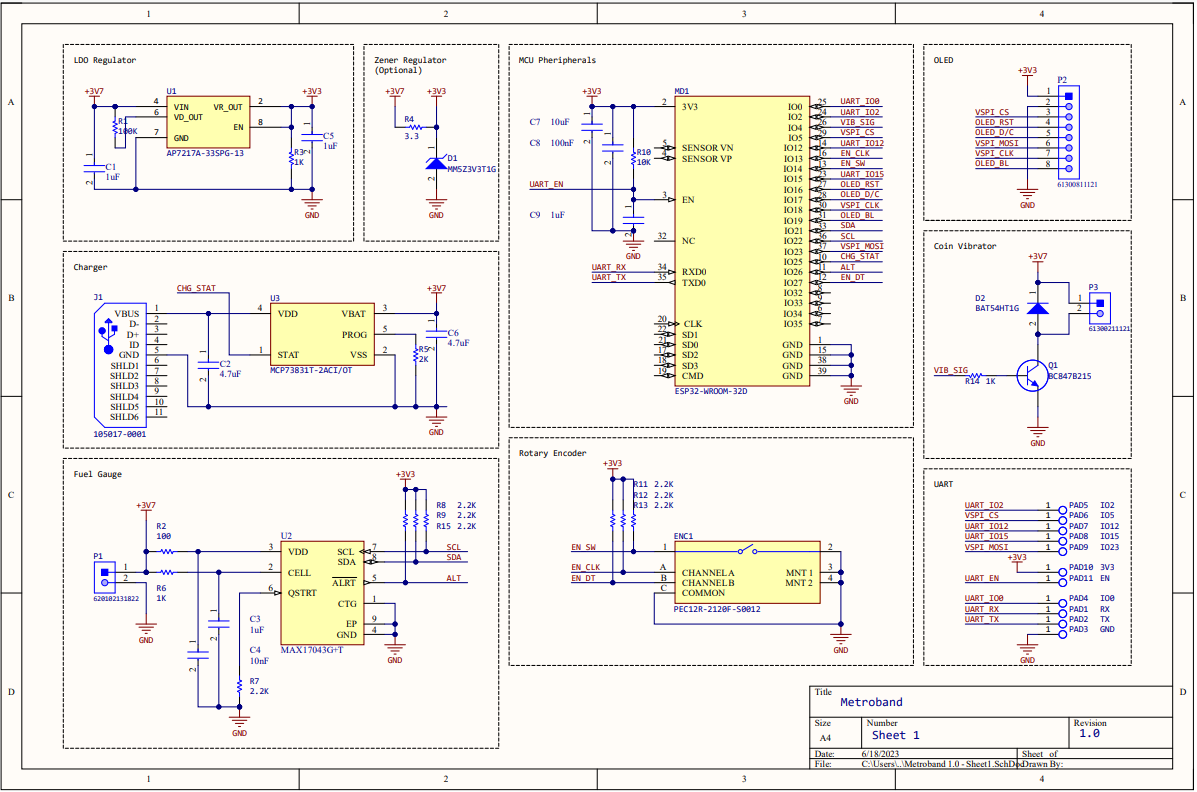
\includegraphics[width=15cm]{3.png}};
                \end{tikzpicture}
                \caption{Schematic Diagram}
                \label{schematic}
            \end{figure}
        \begin{figure}[!htb]
                \centering
                \begin{tikzpicture}
                    \node at (0.5,-0.2){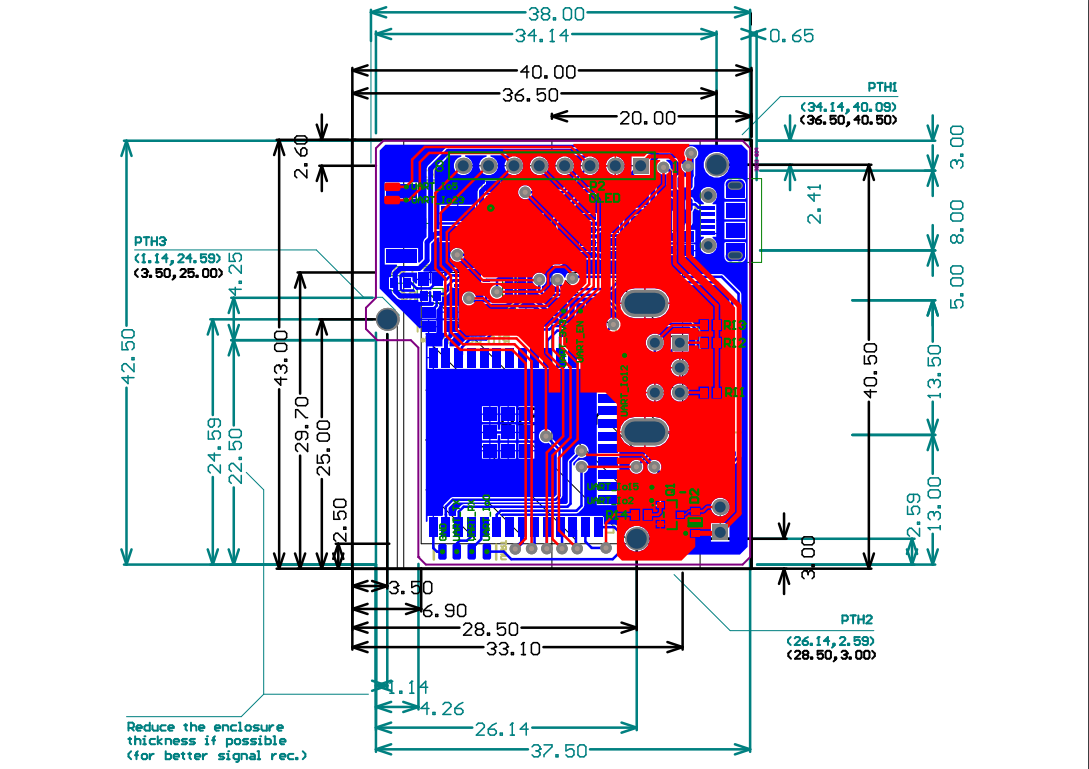
\includegraphics[width=12cm]{4.png}};
                \end{tikzpicture}
                \caption{PCB overview}
                \label{pcb}
            \end{figure}
        \begin{figure}[!htb]
                \centering
                \begin{tikzpicture}
                    \node at (0.5,-0.2){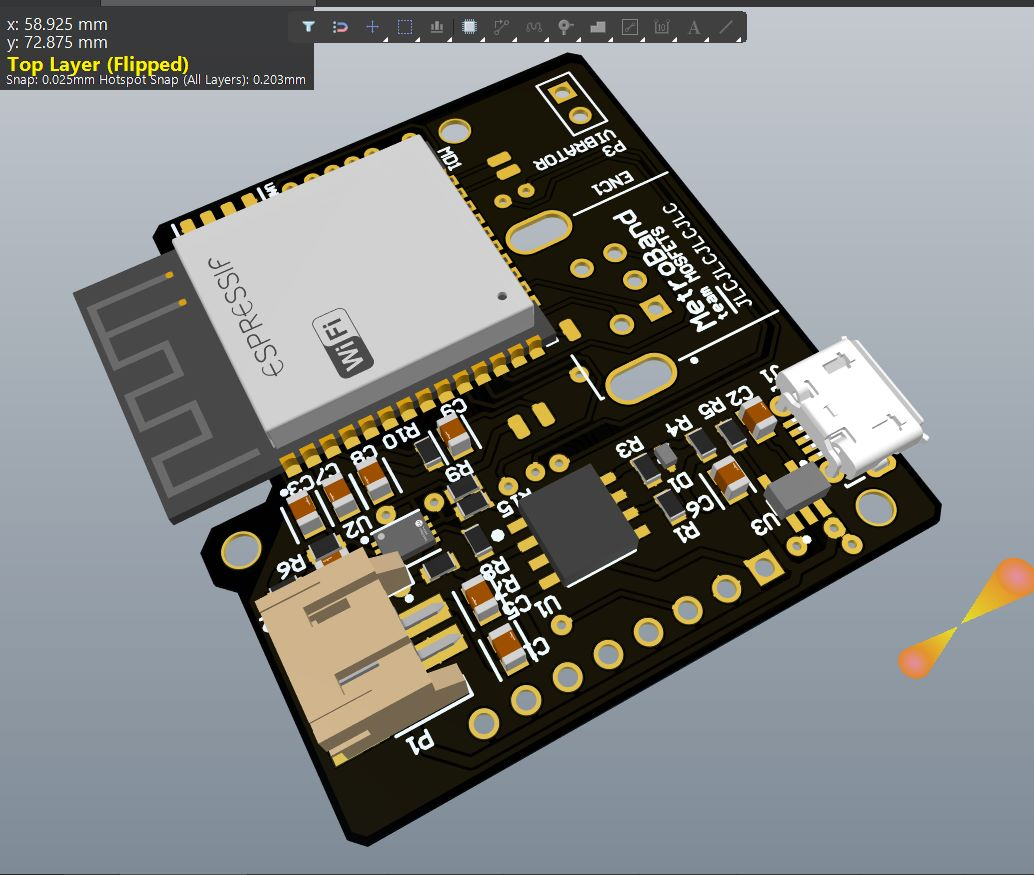
\includegraphics[width=12cm]{5.jpeg}};
                \end{tikzpicture}
                \caption{3D view of the PCB}
                \label{pcb3d}
            \end{figure}
        The circuit diagram of the product is shown below in Figure \ref{schematic}. It was designed with a voltage regulator as the battery gives a voltage of 4.2V when fully charged, and the ESP32 requires 3.6-2.2V. Although the IC was included in the circuit, due to predictions of local unavailability of the ICs we included a slot for a zener diode of 3.3V to be soldered as well.\\
        
        Several modifications were done for the display, as we chose a TFT display rather than an OLED display.\\
        
        All the functionalities of the circuit are controlled by the rotary encoder and its inbuilt push-button (manually) and via bluetooth.\\
        
        The PCB in size is 42.5mm x 38mm as it requires to be small enough to fit on a wrist. Hence it was required to use SMD components. also the required clearances for the antenna of the ESP32 were kept. ESP32 was planned to be programmed with the UART converter of a development board, and for this purpose several test pads were kept so wires could be soldered and it desoldered at the last minute.

        \subsection{Coding}
        For coding we used the ESP IDF. We carried out the tasks separately in the singular core rather than carrying all the tasks in a singular loop while adjusting their priorities.
        Also we had to use multiple libraries in order to code the parts related to bluetooth, display and other functions of the ESP32. Further, we had to design the bitmap of the icons as well as the numbers, as we used a 16-segment display font.

        \subsection{Enclosure Design}
        The enclosure was designed using SOLIDWORKS 2023.We needed to get the enclosure as detailed as possible with minimum dimensions.\\

        \begin{minipage}{\linewidth}
                \centering
                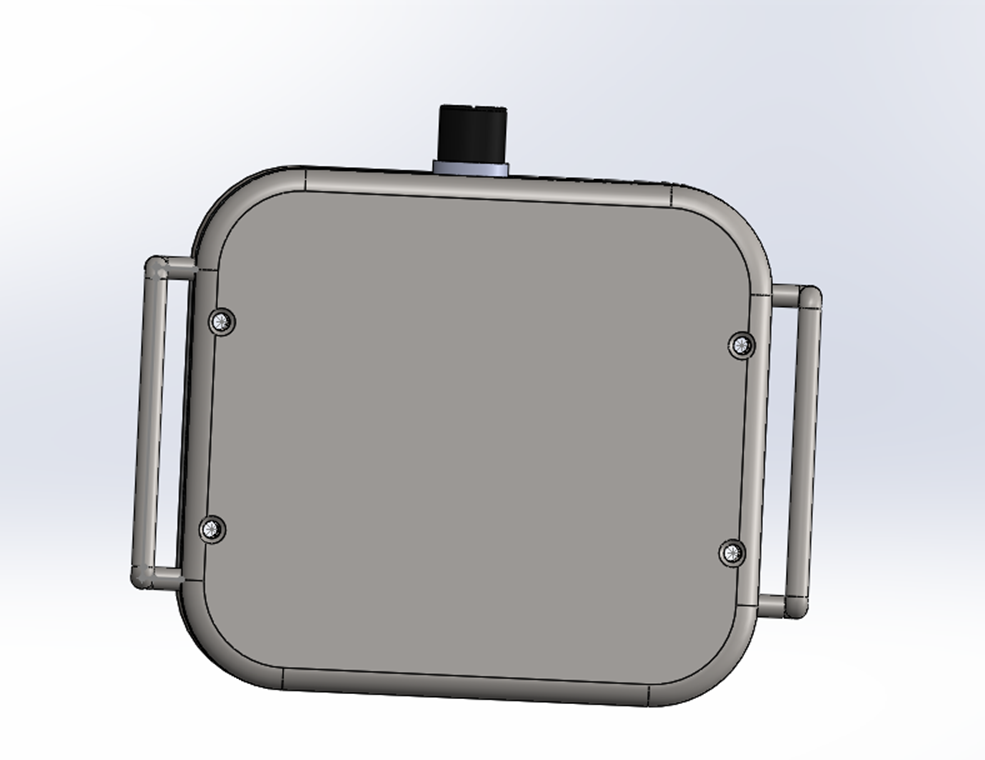
\includegraphics[height=0.4\linewidth]{8.png}
                \hspace{0.005\linewidth}
                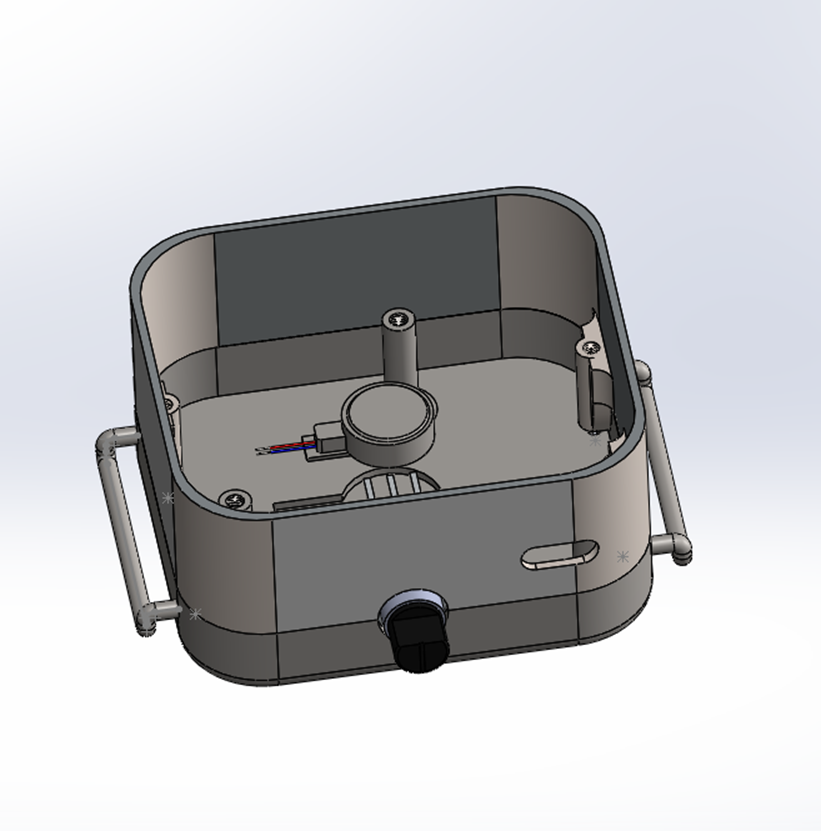
\includegraphics[height=0.4\linewidth]{9.png}
                \hspace{0.005\linewidth}
                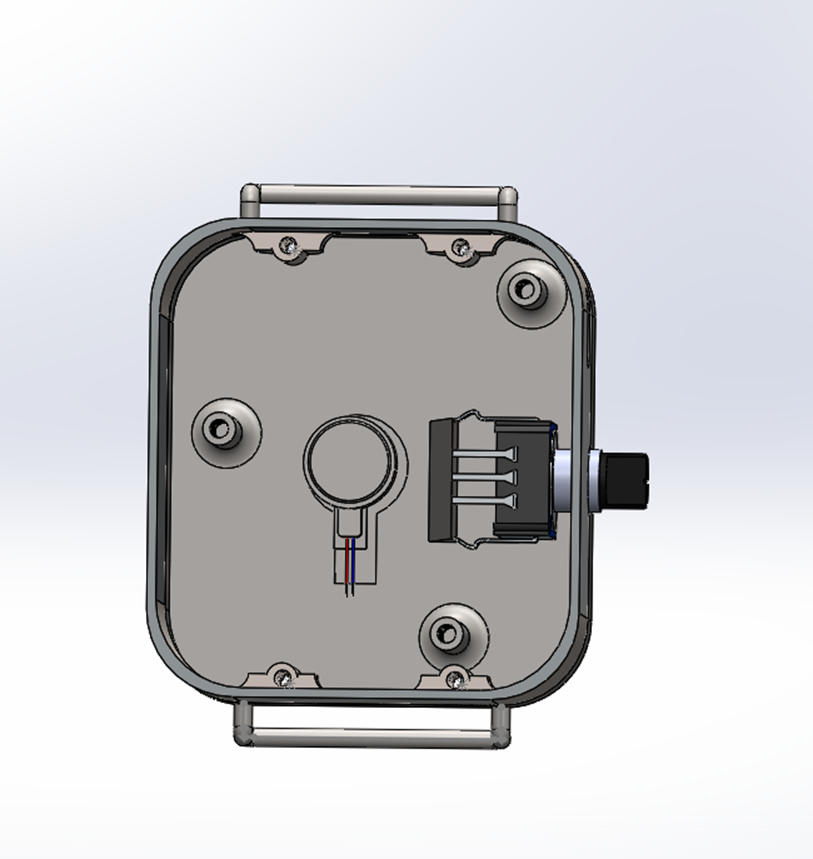
\includegraphics[height=0.4\linewidth]{10.png}
                \captionsetup{justification=centering} % Center-align the caption
                \captionof{figure}{Enclosure SOLIDWORKS design}
            \end{minipage}

        \newpage
        \section{Project Budget}
        \begin{longtable}{|l|r|r|r|}
        
        \hline
        \textbf{Item} & \textbf{Quantity} & \textbf{Unit Price} & \textbf{Price} \\
        \hline
        \endfirsthead
        
        \hline
        \textbf{Item} & \textbf{Quantity} & \textbf{Unit Price} & \textbf{Price} \\
        \hline
        \endhead
        
        \hline
        \endfoot
        
        \hline
        \endlastfoot
        
        Coin vibrator & 1 & RS.300 & RS.300 \\
        Battery & 1 & Rs.450 & Rs.450 \\
        TFT display unit & 1 & Rs.1400 & Rs.1400 \\
        Regulator IC & 1 & Rs.185 & Rs.185 \\
        Fuel gauge IC & 1 & Rs.500 & Rs.500 \\
        Charger IC & 1 & Rs.350 & Rs.350 \\
        mini USB slot & 1 & Rs.150 & Rs.150 \\
        PCB Design and Printing & - & - & Rs.500 \\
        Enclosure Printing & - & - & Rs.760 \\
        Padding and Straps & - & - & Rs.250 \\
        Resistors & 6 & - & Rs.50 \\
        Capacitors & 8 & - & Rs.50 \\
        Transistor & 1 & Rs.5 & Rs.5 \\
        Esp 32 module & 1 & Rs.700 & Rs.700 \\
        Rotary Encoder & 1 & Rs.350 & Rs.350 \\
        \hline
        \textbf{Total cost for components} & - & - & \textbf{Rs.5995.00} \\
        \textbf{Number of units} & - & - & \textbf{200} \\
        \textbf{Marketing and sales cost} & - & - & \textbf{Rs.10,000} \\
        \textbf{Profit per unit} & - & - & \textbf{Rs.5000} \\
        \textbf{Product price} & - & - & \textbf{Rs.10,000} \\
        \hline
        \end{longtable}
        

        \section{Future Developments}
        \subsection{Size}
        Currently we have identified that the size of the prototype could be a hindrance for some musicians. Hence we intend to reduce the size of the watch to a wearable size. In order to do this we have come across few methods:
        \begin{itemize}
                \item Using a TFT display without the breakout PCB, as the PCB and the pin headers add 3 mm to the height
                \item By using a smaller rotary encoder which is usually used in applications such as smartwatches, we can further reduce the height
                \item By resorting to a further compact design in designing the PCB, and outsourcing the soldering of components to a ‘pick and place’ services provider, the length and width of the apparatus could be reduced
                \item By choosing a thinner battery, the height could be further reduced
        \end{itemize}

        \subsection{Display}
        Currently we have included a 1.44 inch TFT. As this does not cover the complete front face of the watch, we have identified that it would be better to choose a display slightly larger than the current display, which would be rather aesthetically pleasing to the consumer.\\
        Further, the current display elements are designed in such a way so they are reminiscent of the classic ‘Vacuum Fluorescent Displays’, which would be further improved in the design phase to further resemble.

        \subsection{Vibration Intensity}
        For musicians who play rather delicate instruments such as piano or violin, more subtle vibrations are required. And some users would need a user set vibration intensity for the device to vibrate with. For this, we have identified using a PWM signal with an adjustable duty cycle as a solution. The code will be changed accordingly to achieve this, and a setting to change the intensity would be added to the mobile app. 

        \subsection{USB C port}
        Recently, USB-C has become the standard connector for the devices. Hence USB-C cables are becoming more available. Hence by changing the Micro-USB to a USB-C port, we give the consumer the opportunity to use any charging cable as they would please.

        \subsection{Battery}
        With the current battery, the device’s charge remains up to 5 hours when in use. This could be further improved with using a battery with a better capacity, while retaining (or preferably reducing) the size.

        \subsection{Enclosure}
        The enclosure will have a design makeover, with a newer, more attractive design which suits the modern market. The straps would be replaced with more comfortable silicone straps, and the body would have a more sleek design.

        \subsection{Mobile Application}
        The app is to be  featured with additional features. The vibration intensity can be set by the mobile app which will make it feasible for playing different instruments that require different vibration intensities. Moreover, presets can be saved in the mobile app so that the Metroband can help the musicians in playing music that changes its beat in-between or  gradually. Additionally, playlists can be saved in the mobile app. Also the UI design will be improved.


        \section{Marketing, Sales, and After-sales}
        \subsection{Marketing}
        We’ll be focusing our marketing effort on musicians, music students, choirs and orchestras. The silent and convenient alternative to traditional metronomes, allowing for uninterrupted practice sessions will be highlighted which will be offered by the “Metroband”.\\
        
        We’ll be engaging with online communities, forums, Facebook, WhatsApp, twitter and other social media groups that are dedicated to musicians and music enthusiasts. We will be participating in discussions, sharing valuable insights while promoting the “Metroband” as a useful tool not only for the musicians seeking an innovative way to keep the BPM without the noise, but also for the musicians with hearing disorders to keep up their beat in time.\\
        
        We’ll be also creating engaging creative videos that demonstrate the functionality, the benefits and the need of the “Metroband” for the musicians. Moreover, how the wristband can be synchronized with various instruments and used during practice sessions can be shown. These videos will be shared on our website and social media platforms.\\
        
        Also we were able to present our product at the EXMO exhibition which was held on 27th to 29th of July, which gave a great exposure for our product, which also gave us the opportunity to connect with potential investors.

        \subsection{After-sales}
        Encourage the customers to provide feedback and testimonials about their experience using the “Metroband”. Positive reviews can be highlighted and posted on social media channels to gain the trust and attract new customers. Negative reviews will be carefully comprehended, and prompt actions will be taken to resolve them.\\
        
        Because the ESP32 board is used here we are able to code it so that it is able to receive over the air firmware updates (OTA updates). Because of this even more functionalities can be added even after the sale of the product.\\
        
        The product's disposability is also taken into consideration. There will be detailed instructions on how to properly dispose of the wristbands, including details on recycling possibilities. Any harmful or poisonous materials can be reused or given to electronic shops for reuse because they are not used in the electronic component. Additionally, details will be provided on how customers can return straps so that we can recycle or re-purpose them.\\

        \section{Task Allocation}

        \begin{itemize}
            \item \textbf{Nawarathna D.M.G.B}
                \begin{itemize}
                    \item Coding
                    \item PCB Design
                    \item Vibrating Motor Module
                \end{itemize}

            \item \textbf{Senevirathne I.U.B}
                \begin{itemize}
                    \item OLED Display Module
                    \item Web App Development
                    \item Budget Management
                    \item Enclosure Design
                \end{itemize}

            \item \textbf{Silva L.J.J.P}
                \begin{itemize}
                    \item Microcontroller and the Peripherals
                    \item Enclosure Design
                    \item Market Research
                \end{itemize}
        
            \item \textbf{Silva M.K.Y.U.N}
                \begin{itemize}
                    \item PCB Design
                    \item Schematic
                    \item Fuel Gauge 
                    \item Coding
                \end{itemize}
        \end{itemize}

        
        
        

        
\end{document}